\documentclass[]{article}
\usepackage{amssymb}
\usepackage{amsmath}
\usepackage[utf8]{inputenc}
\usepackage{graphicx}
\usepackage{booktabs}
\usepackage{listings}
\usepackage{color}
\usepackage{tabularx}
\usepackage{hyperref}

\definecolor{dkgreen}{rgb}{0,0.6,0}
\definecolor{gray}{rgb}{0.5,0.5,0.5}
\definecolor{mauve}{rgb}{0.58,0,0.82}

\lstset{frame=tb,
	%language=C++,
	aboveskip=3mm,
	belowskip=3mm,
	showstringspaces=false,
	columns=flexible,
	basicstyle={\small\ttfamily},
	numbers=none,
	numberstyle=\tiny\color{gray},
	keywordstyle=\color{blue},
	commentstyle=\color{dkgreen},
	stringstyle=\color{mauve},
	breaklines=false,
	breakatwhitespace=true,
	tabsize=2
}


\title{FYS-STK4155 H20 - Project 2:\\A Study of Stochastic Gradient Descent and its Application in Linear and Logistic Regression Methods and Feed-Forward Neural Networks}
\author{Olav Fønstelien}

\begin{document}
\maketitle

\begin{abstract}
%The abstract gives the reader a quick overview of what has been done and the most important results. Try to be to the point and state your main findings. It could be structured as follows 
% - Short introduction to topic and why its important 
% - Introduce a challenge or unresolved issue with the topic (that you will try to solve) 
% - What have you done to solve this 
% - Main Results 
% - The implications

In this report we give a concise presentation of the mathematical derivation of Stochastic Gradient Descent (SGD) and Feed-Forward Neural Networks (FFNN), a simple type of artificial neural network. We show that SGD may be used with linear regression methods like Ordinary Least Squares (OLS) and Ridge, but that its $R_2$ score generally is somewhat poorer than that of traditional OLS with matrix inversion, at 0.63 vs. 0.69. We also show that a simple implementation of a FFNN performs well on the simplified MNIST dataset available through \lstinline|sklearn|, with 98 \% accuracy vs. 99 \% for the widely known \lstinline|sklearn.neural_network.MPLClassifier|.

Please visit my GitHub repository \url{https://github.com/fonstelien/FYS-STK4155/tree/master/project2} for the Python source code developed for this report.

\end{abstract}

\section{Introduction} \label{intro}
%When you write the introduction you could focus on the following aspects
% - Motivate the reader, the first part of the introduction gives always a motivation and tries to give the overarching ideas
% - What I have done
% - The structure of the report, how it is organized etc

% Refer to project 1 and the inefficiency and limitations of linear regression -> SGD + logistic regression -> limits of logistic regression -> neural networks
In \cite{project1} we studied linear regression methods. We saw that for the Ordinary Least Squares (OLS) and Ridge methods we had to calculate a matrix product on the form $(\mathbf{X}^\intercal \mathbf{X} + \lambda \mathbf{I})^{-1} \mathbf{X}^\intercal$ in order to obtain the coefficient estimates $\mathbf{\hat{\beta}}$ ($\lambda = 0$ for OLS). As we saw in \cite{project1}, the matrix inversion operation may be numerically unstable, and if we need a large number of samples to approximate the function, this operation becomes computationally demanding or even infeasible. 

The Stochastic Gradient Descent method (SGD) deals with both of these problems. It still requires calculating $\mathbf{X}^\intercal \mathbf{X}$, but since it determines the coefficient estimates $\mathbf{\hat{\beta}}$ iteratively on so-called \textit{mini batches} which can be kept in the higher levels of cache, the operation becomes less computationally demanding. The inversion operation is avoided all-together. 

SGD is useful in other methods as well. SGD can be used in logistic regression methods, which lets us solve \textit{classification problems} where we predict the outcome of an event as the one most likely of several possible \textit{classes} of outcomes. For these problems, linear regression methods are unsuitable. Logistic regression again is unsuitable for the class of problems where the decision boundary between features and outcomes is non-linear, like the \textit{XOR} (exclusive or) logical operator. For these problems, Artificial Neural Networks (ANNs) can be used, for which SGD forms an integral part of the learning process.

In this report we will develop methods for SGD in linear and logistic regression methods, as well as the Feed-Forward Neural Network, and give outlines for their implementation in a computer program. We will aim our mathematical derivations on the implementation in a array programming environment. We will study the performance of our methods on linear regression problems and both binomial and multinomial classification problems, using datasets which are well known in the literature, namely the Wisconsin Breast Cancer dataset and a simplified form of the MNIST dataset of handwritten figures 0 to 9 \cite{skl-datasets}.

We begin in Section \ref{methods} with the mathematical derivations, first of Stochastic Gradient Descent, and then the Feed-Forward Neural Network. Then we move on Section \ref{results}, where we study the results and performance of the methods. We end by summing up our findings, with some suggestions for further studies in Section \ref{conclusion}.

\clearpage
\section{Methods} \label{methods}
% - Describe the methods and algorithms
% - You need to explain how you implemented the methods and also say something about the structure of your algorithm and present some parts of your code
% - You should plug in some calculations to demonstrate your code, such as selected runs used to validate and verify your results. The latter is extremely important!! A reader needs to understand that your code reproduces selected benchmarks and reproduces previous results, either numerical and/or well-known closed form expressions.

In this section we will develop methods for solving regression and classification problems with traditional linear and logistic regression methods, as well as Feed-Forward Neural Network, a simple type of ANN. In the outline I will use matrix notation where possible, since this closely resembles the implementation in a computer programming environment with array programming capabilities like native MATLAB, C++ with the \lstinline|armadillo| lib or Python with the \lstinline|numpy| module, which I will use.

\subsection{Stochastic Gradient Descent}
Stochastic Gradient Descent is a numerical method for minimizing the cost function of a mathematical optimization method like OLS or logistic regression, where the minimization is done in an iterative, stochastic approach on a selection of the full set of samples. That is; given a cost function $\mathcal{C}(\mathbf{\beta})$, where $\mathbf{\beta} \in \mathbb{R}^p$, SGD lets us solve the problem
\begin{equation}
	\frac{\partial \mathcal{C}(\mathbf{\beta})}{\partial \mathbf{\beta}} = \mathbf{0},
\end{equation}
where a closed-form solution is otherwise not available, or computationally expensive, and by using only a sub-set of the samples in each iteration. It is based on the iterative application of Newton-Raphson's method on the coefficient vector $\mathbf{\beta}$, such that
\begin{equation} \label{newton-raphson}
	\mathbf{\beta}^{(i+1)} = \mathbf{\beta}^{(n)} - [\mathbf{H}^{(i)}]^{-1}\mathbf{g}^{(i)},
\end{equation}
where $\mathbf{g}$ is the gradient of the cost function and $\mathbf{H}$ is its Hessian matrix, each given by
\begin{equation}
	\mathbf{g}^{(i)} = \frac{\partial \mathcal{C}(\mathbf{\beta}^{(i)})}{\partial \mathbf{\beta}} \quad \text{, and} \quad 
	\mathbf{H}^{(i)} = \frac{\partial^2 \mathcal{C}(\mathbf{\beta}^{(i)})}{\partial \mathbf{\beta} \partial \mathbf{\beta}^\intercal}.
\end{equation}
Equation (\ref{newton-raphson}) can be deduced from the Taylor expansion of $\mathcal{C}(\mathbf{\beta})$ around $\mathbf{\beta}^{(i+1)} - \mathbf{\beta}^{(i)}$. See \cite{fys-stk4155-notes} for a thorough outline of this.

Calculating the Hessian and inverting it is an expensive and numerically volatile operation, so our approach will be to replace it by a scalar $\eta$, the so-called \textit{learing rate}, such that $\mathbf{H}^{-1} \rightarrow \eta$. Equation (\ref{newton-raphson}) thus becomes
\begin{equation} \label{newton-raphson-eta}
	\mathbf{\beta}^{(i+1)} = \mathbf{\beta}^{(i)} - \eta \mathbf{g}^{(i)}.
\end{equation}

Finding the \textit{best} $\eta = \hat{\eta}$, such that $\mathbf{\beta}^{(i+1)} = \mathbf{\hat{\beta}}$ again involves calculating the Hessian, unfortunately \cite{fys-stk4155-notes}; 
\begin{equation}
	\hat{\eta} = \frac{\mathbf{g}^\intercal \mathbf{g}}{\mathbf{g}^\intercal \mathbf{H} \mathbf{g}}.
\end{equation}
However, the cost function $\mathcal{C}(\mathbf{\beta})$ is guaranteed to be convex for linear and logistic regression problems, implying a positive definite $\mathbf{H}$ \cite{murphy2012machine}. Therefore, as long as we select $\eta < 2/\lambda_{max}$, where $\lambda_{max}$ is the largest eigenvalue of the Hessian matrix, Equation (\ref{newton-raphson-eta}) will converge towards $\mathbf{\hat{\beta}}$. Again, $\lambda_{max}$ will remain unknown to us; but knowing that if we select a $\eta$ which is not too large, a solution will be found, we base our approach on trial and error. 

\vspace{5mm}

The next problem then becomes to decide when to stop the search for $\mathbf{\hat{\beta}}$. One solution is to stop when the difference between the iterations becomes smaller than some defined value, $||\mathbf{\beta}^{(n+1)} - \mathbf{\beta}^{(n)}||_2 \le \varepsilon$. Another, which we will use here, is simply to define a number of iterations, and extract the solution thereafter. This might seem a little inaccurate, maybe, but works well since the direction of $\mathbf{g}$ is always towards the global minimum, and $|\mathbf{g}| \rightarrow 0$ when $\mathbf{\beta} \rightarrow \mathbf{\hat{\beta}}$, which means that if we come close to $\mathbf{\hat{\beta}}$, the final approximation $\mathbf{\beta}^{(final)} \approx \mathbf{\hat{\beta}}$.

A further refinement to this is to incrementally decrease $\eta$ for each iteration towards $\mathbf{\hat{\beta}}$; that is to let $\eta \rightarrow \eta^{(i)} = f(i)$, such that $\eta^{(i+1)} < \eta^{(i)}$. This increases the stability of the method since it allows us to even have $\eta^{(0)} > 2/\lambda_{max}$ and still get convergence.

Two such \textit{learning schedules} $\eta^{(i)} = f(i)$ are the \lstinline|invscaling| schedule in Python's \lstinline|scikit-learn| module \cite{skl};
\begin{equation} \label{invscaling}
	\eta^{(i)} = \frac{\eta^{(0)}}{i^k},
\end{equation}
and another one suggested by Geron in \cite{geron2019hands};
\begin{equation} \label{geron}
	\eta^{(i)} = \frac{t_0}{i + t_1}.
\end{equation}
Here the factors $k, t_0, t_1$ are user defined. Figure \ref{fig:learning_schedules} shows each learning schedule with some selections for the user-defined factors over the 100 first iterations.

\vspace{5mm}

Calculating the gradient of the cost function $\mathbf{g}$ in Equation (\ref{newton-raphson-eta}) may prove computationally demanding if the data set is large. The gradient of the logistic regression method cost function, for instance, would require that we calculate the matrix product $\mathbf{X}^\intercal \mathbf{P}$ in each iteration. In SGD, we select a subset of the samples by a stochastic process, and calculated an approximated gradient based on this subset or mini batch. The standard deviation of the gradient's expectation value relative to the number of samples $n$ follows the relation \cite{fys-stk4155-notes}
\begin{equation}
	\sigma_g \sim \frac{1}{\sqrt{n}},
\end{equation}
which means that if we collect a mini batch of 100 from a data set of 1000 samples, the standard deviation will only increase by a factor of 3, but the computation of each iteration will run 10 times faster.

Another great advantage of only approximating the gradient on a mini sample is the decreased risk of getting stuck in a local minimum or saddle point, where $\mathbf{g} \rightarrow 0$, but $\mathbf{\beta} \neq \mathbf{\hat{\beta}}$. This is especially useful in neural network applications, where it is not given that we have a convex cost function.

The implementation of SGD is outlined in Listing \ref{lst:sgd}. An \lstinline|epoch| is defined as a full run through the full set of samples. The \lstinline|learning_schedule()|s could be as in Equations (\ref{invscaling}) and (\ref{geron}). 

\vspace{5mm}

The \lstinline|cost_function_gradient()|s that we will use in this report are Mean Squared Error (MSE), used in OLS and Ridge regression methods; and Cross Entropy (CE), used in the logistic regression method. MSE cost function gradient is given by
\begin{equation} \label{cost-mse}
	\mathbf{g}_{mse}^{(n)} = \frac{\partial \mathcal{C}_{mse}^{(n)}}{\partial \mathbf{\beta}} = \frac{1}{n} ((\mathbf{X}^\intercal \mathbf{X}) \mathbf{\beta}^{(n)} - \mathbf{X}^\intercal \mathbf{y}) + \lambda \mathbf{\beta}^{(n)},
\end{equation}
where $\mathbf{y}$ is the response variable vector and $\lambda$ is the $L_2$ regularization parameter \cite{project1}. 

%\begin{minipage}{\linewidth}
\begin{lstlisting}[caption={Stochastic Gradient Descent algorithm. Cost function gradients and learning schedules may be defined independently of the implementation of SGD. This implementation runs for \lstinline|epochs*batches| iterations, and does not sense if or when it converges.},label={lst:sgd}] [!ht]
	// Declarations
	betas = "initial coefficient values"
	epochs = "number of runs through data set"
	batches = "number of mini batches"
	iteration_number = 0
	
	// Inputs
	data = "the design matrix"
	targets = "the response variables"
	
	// SGD process	
	FOR i = 1...epochs DO
		shuffle(data, targets)
		FOR j = 1...batches DO
			data_batch, targets_batch = "draw mini batch from full set w/o replacement"
			iteration_number++
			eta = learning_schedule(iteration_number, args...)
			grad = cost_function_gradient(data_batch, targets_batch)
			betas = betas - eta*grad
		END FOR
	END FOR
\end{lstlisting}
%\end{minipage}

The CE cost function gradient is given by
\begin{equation} \label{cost-mse}
	\mathbf{g}_{ce}^{(n)} = \frac{\partial \mathcal{C}_{ce}^{(n)}}{\partial \mathbf{\beta}} = \frac{1}{n} (\mathbf{X}^\intercal \mathbf{P}^{(n)} - \mathbf{X}^\intercal \mathbf{Y}) + \lambda \mathbf{\beta}^{(n)}.
\end{equation}
Here, $\mathbf{Y} \in \mathbb{R}^{n \times c}$ is the response variable matrix with $n$ samples and $c$ different classes of outcome. Each row $\mathbf{y}_i$ has a single 1, and the rest 0s. Likewise, $\mathbf{P} \in \mathbb{R}^{n \times c}$ is the probability matrix for the $n$ samples and $c$ classes following the \textit{softmax} function:
\begin{equation}
	\mathbf{P} = \mathrm{softmax}(\mathbf{X}'\mathbf{B}).
\end{equation}
$\mathbf{X}'$ is the design matrix with an intercept column added in front $\mathbf{X}' = [\mathbf{1} \quad \mathbf{X}]$. The coefficient matrix $\mathbf{B} \in \mathbb{R}^{(p+1) \times c}$, accounting for the intercept, i.e. the variation in outcomes not explained by the features in $\mathbf{X}$. $\mathbf{B}$ is given by
\begin{equation}
	\mathbf{B} = [\mathbf{\beta}_1 \quad \mathbf{\beta}_2 \quad \cdots \quad \mathbf{\beta}_c], \quad \text{where} \quad \mathbf{\beta}_j = [\beta_{0j} \quad \beta_{1j} \quad \cdots \quad \beta_{pj}]^\intercal.
\end{equation}

Each element $p_{ij}$ in $\mathbf{P}$ is given by
\begin{equation} \label{log-reg-pij}
	p_{ij} = \mathrm{softmax}(\mathbf{X}'\mathbf{B})_{ij} = \frac{\mathrm{exp}(\mathbf{x}_i'\mathbf{\beta}_j)} {\sum_{c}\mathrm{exp}(\mathbf{x}_i'\mathbf{\beta}_c)},
\end{equation}
and the sum of each row $\mathbf{p}_i$ in $\mathbf{P}$ is 1; $\sum_{j} p_{ij} = 1$.

\vspace{5mm}

In Figure \ref{fig:demo_lin_log_reg} we see a demonstration on some mock-up cases for each of the regression methods OLS and Rdge with SGD, and logistic with SGD. For the linear regression cases, a simple linear function with some noise has been used; $y_i = 1 + 2x_i + \varepsilon_i$, where $\mathbf{\epsilon} \sim \mathcal{N}(0, 0.75^2)$, and samples $n=100$. We see that both methods make the fit quite well after 20 epochs and 10 mini batches with constant learning schedule with $\eta = 0.5$ for OLS and $\eta = 0.7, \lambda=0.1$ for Ridge.

The logistic regression classification problem mock-up is shown in Table \ref{tab:logreg-demo}. The design matrix $\mathbf{X}'$ is generated by adding some noise to an identity matrix of dimension $3 \times 3$, and adding the intercepts. Each of the three cases represent distinct outcomes, $\mathbf{Y}$. To the right in Figure \ref{fig:demo_lin_log_reg} we see that when we use the result of the logistic regression $\mathbf{B}$ to fit to $\mathbf{X}'$, correct outcomes are predicted with high confidence in each case.

\begin{figure}[!htb]
	\centering
	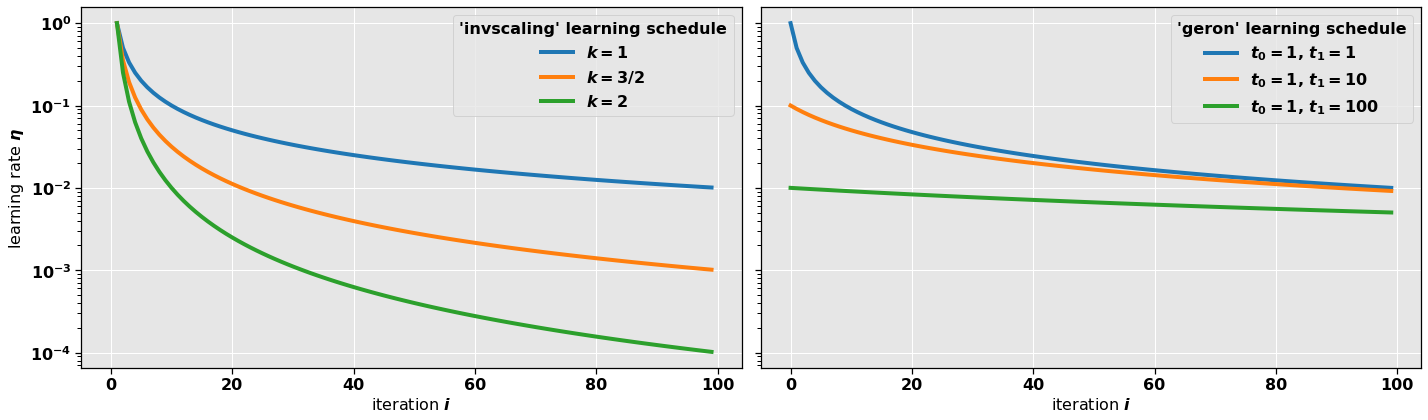
\includegraphics[width=1\linewidth]{learning_schedules.png}
	\caption{Two different learning schedules over the 100 first iterations. To the left we see the \lstinline|invscaling| schedule in Python's \lstinline|scikit-learn| module, as given in Equation (\ref{invscaling}). To the right we see the simple schedule suggested by Geron, as given in Equation (\ref{geron}).}
	\label{fig:learning_schedules}
\end{figure}

\begin{figure}[!htb]
	\centering
	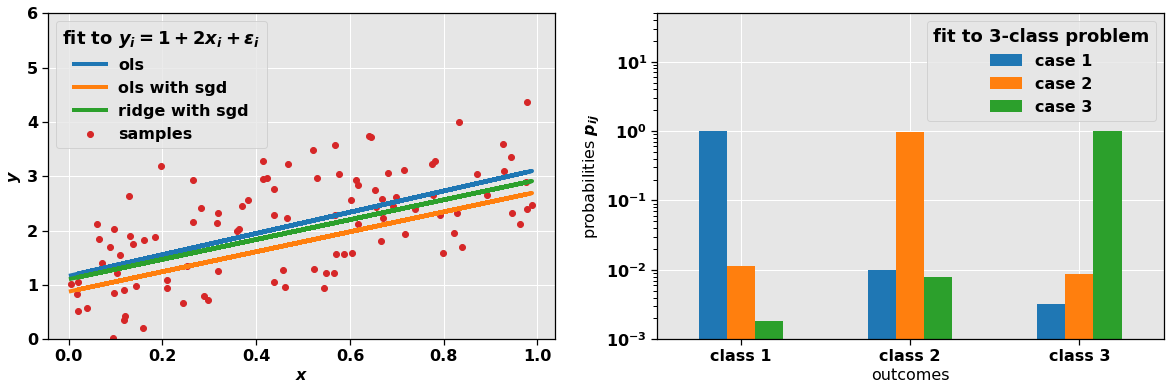
\includegraphics[width=1\linewidth]{demo_lin_log_reg.png}
	\caption{Demonstration of linear regression to the left, and logistic regression to the right using the SGD method. For linear regression, the fit is guaranteed to be best for the simple OLS case since the model we try to fit corresponds exactly to to the function which generated the samples, but we see that both OLS with SGD and Ridge with SGD approach simple OLS. For logistic regression, a mock-up model of a $3 \times 3$ design matrix $\mathbf{X}$ plus intercept is fitted to a $3 \times 3$ one-hot matrix $\mathbf{Y} = \mathbf{I}$. See Table \ref{tab:logreg-demo}. To generate the result, $\mathbf{X}$ has been fed into the softmax function together with the result of the regression fit $\mathbf{B}$ (Equation (\ref{log-reg-pij})). We see that we pick the right class with high confidence in each case.}
	\label{fig:demo_lin_log_reg}
\end{figure}



\begin{table}[!ht]
	\caption{Mock-up classification problem for demonstration of logistic regression. The table has three cases or samples 1,2,3, which are represented with the design matrix $\mathbf{X}'$ in the middle and the one-hot response variable matrix $\mathbf{Y}$ to the right. See the result of the demo to the right in Figure \ref{fig:demo_lin_log_reg}.}
	\label{tab:logreg-demo}
	\begin{center}
		\begin{tabular}{r|rrrr|rrr}
			\toprule
			case &  intercept &     $p_1$ &     $p_2$ &     $p_3$ &  class 1 &  class 2 &  class 3 \\
			\midrule
			1 &          1 &  1.548814 &  0.715189 &  0.602763 &        1 &        0 &        0 \\
			2 &          1 &  0.544883 &  1.423655 &  0.645894 &        0 &        1 &        0 \\
			3 &          1 &  0.437587 &  0.891773 &  1.963663 &        0 &        0 &        1 \\
			\bottomrule
		\end{tabular}
	\end{center}
\end{table}


\subsection{Feed-Forward Neural Network}
The linear and logistic regression methods each have their well-defined set of problems where they come to use; regression and classification, respectively. Artificial Neural Networks is another method, which is can be used for both types of problems, including classification problems with non-linear decision boundaries, like the XOR logical operator, or binary number representation. In this report we study a type of ANN called Feed-Forward Neural Network (FFNN).

Figure \ref{fig:ann-illustration} gives an illustration of a typical FFNN. The layers consist of one or more \textit{nodes} with a \textit{activation function}. Each node-to-node connection has a \textit{weight}, and the input to each node's activation function is the weighted sum of the inputs from all the nodes in the former layer, plus a node-specific \textit{bias}. Except for in the input layer, where the design matrix $\mathbf{X}$ is fed in, all the activation functions are non-linear. This gives the network a highly non-linear behavior. The output of the first hidden layer is thus a non-linear transformation of the information in the input layer, and this process is repeated in the succeeding layers, including the output. At the output layer, the output is evaluated against a suitable cost function, and the error is back-propagated up through the network, which regulates the incremental update of weights and biases. This \textit{training} process is then repeated for a given number of times, or until we have convergence.

\vspace{5mm}

What follows now is a mathematical derivation of the feed-forward, back-propagation and variable update of an FFNN. It is in large part based on \cite{fys-stk4155-notes}, but translated into full matrix notation for simpler implementation in an array programming environment. The reader is encouraged to refer to this source for a thorough, general outline.

As indicated above, the input layer in our FFNN does not have an activation function, it only passes the design matrix $\mathbf{X}$ on to the first hidden layer. If we let $\mathbf{X} \in \mathbb{R}^{n \times p}$, the input layer will have $p$ nodes which are all connected to the $m$ nodes of layer 1, the first hidden layer. Layer 1's weight matrix $\mathbf{W}_1 \in \mathbb{R}^{p \times m}$ is then given as
\begin{equation}
	\mathbf{W}_1 = 
	\left[\begin{array}{cccc}
		w_{11} &w_{12} & \cdots &w_{1m} \\
		w_{21} &w_{22} & \cdots &w_{2m} \\
		\vdots &\vdots &\vdots  &\vdots \\ 
		w_{p1} &w_{p2} & \cdots &w_{pm} \\
	\end{array} \right]_{(1)},
\end{equation} 
and its biases are
\begin{equation}
	\mathbf{b}_1 = [b_1 \quad b_2 \quad \cdots \quad b_m]_{(1)}.
\end{equation}
The resulting inputs $\mathbf{Z}_1$ to layer 1's activation function $f_1$ then become
\begin{equation} \label{inputs}
	\mathbf{Z}_1 = \mathbf{X} \mathbf{W}_1 + \mathbf{B}_1, \quad \text{where} \quad \mathbf{Z}_1, \mathbf{B}_1 \in \mathbb{R}^{n \times m}.
\end{equation}
Here, $\mathbf{B}_1$ is the bias matrix; an $n \times m$ matrix with $\mathbf{b}_1 \in \mathbb{R}^m$ repeated in all its $n$ rows.

Layer 1's activation function output $\mathbf{A}_1$ is given by
\begin{equation} \label{outputs}
	\mathbf{A}_1 = f_1(\mathbf{Z}_1) \in \mathbb{R}^{n \times m},
\end{equation}
which is fed into the preceding layer, where this process is repeated. Here we note that this output $\mathbf{A}_1$ is a non-linear transformation of the input $\mathbf{X}$ to the network, which is true also for the remaining layers, including the output layer.

\vspace{5mm}

Let $L$ denote the output layer in our FFNN and $\cal{C}(\mathbf{\theta})$ the cost function of out model, where $\mathbf{\theta}$ may be any variable which influences its value. We evaluate the output of our FFNN against this cost function and update the output layer's weights and biases according to the gradient of the cost function with respect to each set of variables $\mathbf{W}_L, \mathbf{b}_L$;
\begin{equation} \label{wb-update}
\begin{aligned}
		\mathbf{W}_L &\leftarrow \mathbf{W}_L - \eta \frac{\partial \mathcal{C}}{\partial \mathbf{W}_L} \\
		\mathbf{b}_L &\leftarrow \mathbf{b}_L - \eta \frac{\partial \mathcal{C}}{\partial \mathbf{b}_L} \\
\end{aligned},
\end{equation}
where $\eta$ is the learning rate, a hyperparameter.

By the chain rule, it can be shown that
\begin{equation} \label{hadamard}
\begin{aligned}
	\frac{\partial \mathcal{C}}{\partial \mathbf{W}_L} &= 
	\mathbf{A}_{L-1}^\intercal \left(\frac{\partial \mathcal{C}}{\partial \mathbf{A}_L} \circ \frac{df_L}{d\mathbf{Z}_L} \right) \\
	\frac{\partial \mathcal{C}}{\partial \mathbf{b}_L} &= 
	\frac{\partial \mathcal{C}}{\partial \mathbf{A}_L} \circ \frac{df_L}{d\mathbf{Z}_L} \\
\end{aligned},
\end{equation}
where $\circ$ denotes the element-wise Hadamard product. Here we will let $\mathbf{\Delta}_L$ denote this Hadamard product or error term in Equation (\ref{hadamard});
\begin{equation} \label{delta-L}
	\mathbf{\Delta}_L = \frac{\partial \mathcal{C}}{\partial \mathbf{A}_L} \circ \frac{df_L}{d\mathbf{Z}_L}.
\end{equation}
Equation (\ref{wb-update}) now becomes
\begin{equation}
\begin{aligned}
	\mathbf{W}_L &\leftarrow \mathbf{W}_L - \eta \mathbf{A}_{L-1}^\intercal \mathbf{\Delta}_L \\
	\mathbf{b}_L &\leftarrow \mathbf{b}_L - \eta \mathbf{\Delta}_L \\
\end{aligned}.
\end{equation}

The preceding layers up to but not including the input are then updated in a similar fashion by back-propagation of this error up through the network. Again by the chain rule, it can be shown that $\mathbf{\Delta}_{L-1}$ is given by
\begin{equation}
	\mathbf{\Delta}_{L-1} = (\mathbf{\Delta}_L \mathbf{W}_L^\intercal) \circ \frac{df_{L-1}}{d\mathbf{Z}_{L-1}}.
\end{equation}
For the general layer $l \ge 1$, $\mathbf{\Delta}_l$ becomes
\begin{equation} \label{update-deltas}
	\mathbf{\Delta}_{l} = (\mathbf{\Delta}_{l+1} \mathbf{W}_{l+1}^\intercal) \circ \frac{df_l}{d\mathbf{Z}_l},
\end{equation}
and the rule for updating layer $l$'s weights and biases becomes
\begin{equation} \label{update-weights-biases}
\begin{aligned}
	\mathbf{W}_l &\leftarrow (1 - \eta \lambda) \mathbf{W}_l - \eta \mathbf{A}_{l-1}^\intercal \mathbf{\Delta}_l \\
	\mathbf{b}_l &\leftarrow \mathbf{b}_l - \eta \mathbf{\Delta}_l \\
\end{aligned}.
\end{equation}
Here, we have added $\lambda$, the $L_2$ regularization parameter, which follows by the cost function derivation with respect to $\mathbf{W}_L$;
\begin{equation}
	\mathcal{C}' = \mathcal{C} + \frac{\lambda}{2} ||\mathbf{W}_L||_2^2 \rightarrow \frac{\partial \mathcal{C}'}{\partial \mathbf{W}_L} = \frac{\partial \mathcal{C}}{\partial \mathbf{W}_L} + \lambda \mathbf{W}_L.
\end{equation}

\vspace{5mm}

Like for the Stochastic Gradient Descent method discussed in the previous section, the ANN training process is then repeated until convergence, when $||\mathcal{C}(\mathbf{\theta})||_2 \le \varepsilon$, or for a defined number of times, which we will do in this report.

\vspace{5mm}

Neural networks are generally data hungry \cite{fys-stk4155-notes}, so to make the ANN training process as efficient as possible, we will use the Stochastic Gradient Descent method here as well. Another advantage of this approach is that the scattered descent reduces the chance of having the learning process getting stuck in local minima or saddle points. This only involves putting the training process inside the double epochs-batches loop in Listing \ref{lst:sgd}. An outline of the training algorithm is given in Listing \ref{lst:ann-training}.

%\begin{minipage}{\linewidth}
\begin{lstlisting}[caption={Outline of the Feed-Forward Neural Network training process using a Stochastic Gradient Descent scheme. The weights and biases in each layer must be initiated with some value.},label={lst:ann-training},escapeinside={@}{@}] [!t]
	// Declarations
	layers = "collection of layers in the FFNN"
	epochs = "number of runs through data set"
	batches = "number of mini batches"
	iteration_number = 0
	lmd = "L2 regularization parameter"
	
	// Inputs
	data = "the design matrix"
	targets = "the response variables"
	
	// SGD learning process
	FOR i = 1...epochs DO
		shuffle(data, targets)
		FOR j = 1...batches DO
			data_batch, targets_batch = "draw mini batch from full set w/o replacement"
			
			// Feed forward
			layer_outputs = data_batch			
			FOR EACH layer IN layers DO
				"set layer's inputs by @Equation (\ref{inputs})@"
				"set layer's outputs by activation_function() @Equation (\ref{outputs})@"
			END FOR EACH
			
			// Calculate the cost function derivative with respect to output
			// layer outputs and targets
			error = cost_function_derivative("output layer's output", targets_batch)
			
			// Back-propagate the error by @Equations (\ref{delta-L}) and (\ref{update-deltas})@
			FOR EACH layer IN REVERSED(layers) DO
				"set layer's activation function_derivative() with respect to its inputs"
				"set layer's deltas by the back-propagated error"
				error = "error to back-propagate by this layer's new delta and weights"
			END FOR EACH		
			
			// Update weigths and biases
			iteration_number++
			eta = learning_schedule(iteration_number, args...)
			FOR EACH layer IN layers DO
				"update layer's weights by @Equation (\ref{update-weights-biases})@ with step eta, reg. lmd"
				"update layer's biases by @Equation (\ref{update-weights-biases})@ with step eta"
			END FOR EACH
		END FOR
	END FOR
\end{lstlisting}
%\end{minipage}


\vspace{5mm}

The \lstinline|activation_function()|s and \lstinline|activation function_derivative()|s in Listing \ref{lst:ann-training} are very simple non-linear functions. Many types and variants for each type exist, but in this project we limit ourselves to those listed in Table \ref{tab:activation-funcs}.

%, with shapes as shown in Figure XX.

The \lstinline|cost_function_derivative()|s in Listing \ref{lst:ann-training} which we will use in this report are the derivatives with respect to the outputs $\mathbf{A}_L$ of the Mean Squared Error cost function (MSE) and the Cross Entropy cost function (CE). The MSE derivative is given by
\begin{equation}
	\frac{\partial \mathcal{C}_{mse}}{\partial \mathbf{A}_L} = (\mathbf{A}_L - \mathbf{Y}),
\end{equation}
and the CE derivative by
\begin{equation} \label{ce-partial}
	\frac{\partial \mathcal{C}_{ce}}{\partial a_L^{(ij)}} = \frac{a_L^{(ij)} - y^{(ij)}}{a_L^{(ij)} (a_L^{(ij)} - y^{(ij)})}.
\end{equation}
Equation (\ref{ce-partial}) is due to \cite{fys-stk4155-notes}.

\vspace{5mm}

Figure \ref{fig:demo_lin_log_ffnn} shows the simple mock-up regression and classification problems used for SGD demonstration in the previous chapter (Figure \ref{fig:demo_lin_log_reg}) solved by our FFNN.

For the regression problem we fit a network with 1 hidden layer. It has 2 nodes in the input and hidden layers, and 1 node in the output. The activation function is always sigmoid, and the cost function MSE. We have trained this network on $n = 100$ samples $y_i = 1 + 2x_i + \varepsilon_i$ for 100 epochs with mini batches of 10 samples and use $\eta = 0.5$ and the constant training schedule. The 100 samples are then fed back in to make a prediction. We see that as expected the prediction is a non-linear curve, and that it closely follows the OLS fit, but with a slight bend.

Classification is done on the 3-class problem described in Table \ref{tab:logreg-demo}. Again the FFNN has 1 hidden layer, but with 4 nodes in the input and hidden layers, and 3 nodes in the output layer. The hidden layer activation function is ReLU, and the output layer function is softmax, which is suitable for multiclass problems. The cost function is Cross Entropy. We have trained the network for 100 epochs with batch size 1, $\eta = 0.1$ and $L_2$ regularization $\lambda = 0.001$. In the input data cases 1,2,3 correspond to classes 1,2,3, which is also the prediction of our FFNN when the training data is fed back into the network for testing.

\begin{figure}[!htb]
	\centering
	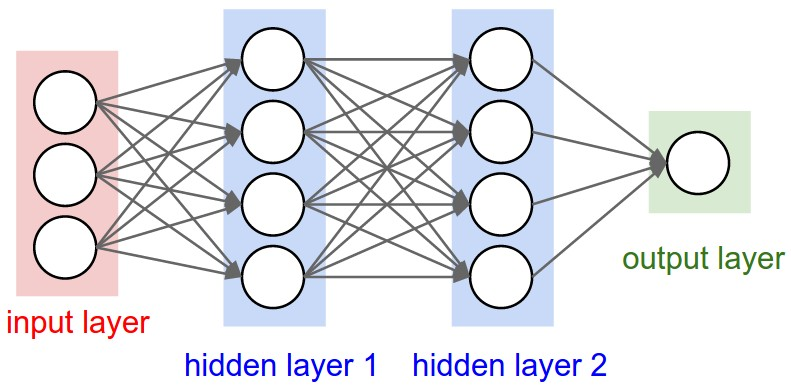
\includegraphics[width=1\linewidth]{ann-illustration.jpeg}
	\caption{ANN with one input layer, two hidden layers, and an output layer. The design matrix is fed into the input layer, and is fed through the hidden layers and the output layer value is evaluated against a cost function. The error is then back-propagated and regulates the adjustment of the weights associated with each node-to-node connection and the bias of each node are in order to make a better fit in the next iteration. To introduce non-linearity, the output of each node is decided by the inputs and bias fed into a non-linear activation function. This network could be used for either regression, or binary classification. Illustration borrowed from \cite{fys-stk4155-notes}.}
	\label{fig:ann-illustration}
\end{figure}

\begin{figure}[!htb]
	\centering
	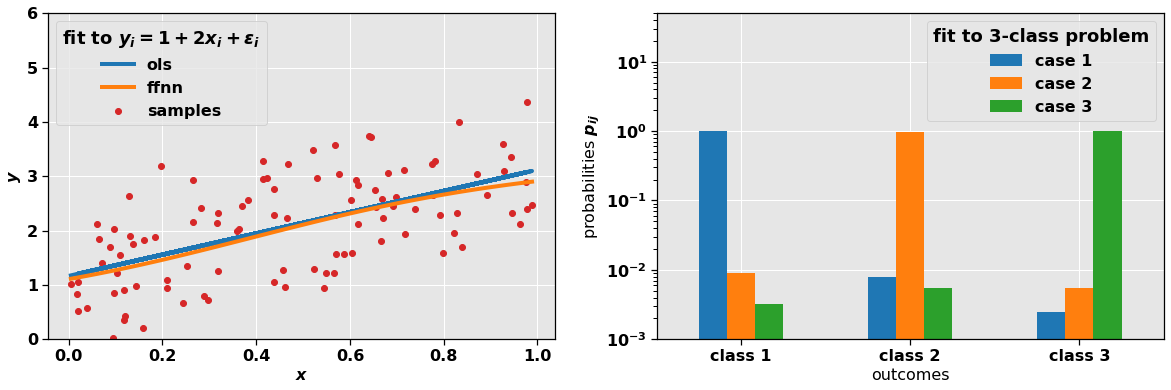
\includegraphics[width=1\linewidth]{demo_lin_log_ffnn.png}
	\caption{Demonstration of FFNN on a simple regression problem to the left, and a simple classification problem to the right. For linear regression, the fit is guaranteed to be best for the simple OLS case since the model we try to fit corresponds exactly to to the function which generated the samples, but we see that the FFNN finds a non-linear fit which closely follows the OLS line. For the classification problem, we predict three cases with three features and three classes of outcome. In the input data cases 1,2,3 correspond to classes 1,2,3, respectively. See Table \ref{tab:logreg-demo} for details. We see that we pick the right class with high confidence in each case. Compare with Figure \ref{fig:demo_lin_log_reg}, which shows the same set of problems solved by linear and logistic regression methods.}
	\label{fig:demo_lin_log_ffnn}
\end{figure}



\begin{table}[!ht]
	\caption{Various activation functions and their derivatives. More variants and types exist, but these are the ones used in this report. ReLU, leaky-ReLU and unit-step derivatives are not defined at $z=0$, but we approximate them as 0 here. Also, the derivative of unit-step is of course always 0, but to progress the learning process it is defined as shown here. The unit-step is usually best suited for classification problems, and softmax especially for multiclass problems. For linear regression problems, sigmoid or one of the ReLUs can be used.}
	\label{tab:activation-funcs}
	\begin{center}
		\begin{tabular}{l|l|l|l}
			\toprule
			name&	$f(z)$&	$f'(z)$&	asymptote \\
			\midrule
			ReLU&	$\mathrm{max}(0,z)$&	1 if $z > 0$; 0 else&	$0,+\infty$ \\
			leaky-ReLU&	$\mathrm{max}(0.01z,z)$&	1 if $z > 0$; 0.01 else&	$-\infty,+\infty$ \\
			unit-step&	1 if $z > 0$; 0 else&	set to 1 if $z > 0$; 0 else&	$0,+1$ \\
			sigmoid&	$1/(1 + e^{-z})$&	$\mathrm{sigmoid}(z)(1 - \mathrm{sigmoid}(z))$	&	$0,+1$ \\
			softmax&	$e^{z_{ij}}/\sum_{c}e^{z_{ic}}$&	$\mathrm{softmax}(z_{ij})(1 - \mathrm{softmax}(z_{ij}))$ &	$0,+1$ \\
			\bottomrule
		\end{tabular}
	\end{center}
\end{table}


\clearpage
\section{Results} \label{results}
% - Present your results
% - Give a critical discussion of your work and place it in the correct context.
% - Relate your work to other calculations/studies
% - An eventual reader should be able to reproduce your calculations if she/he wants to do so. All input variables should be properly explained.
% - Make sure that figures and tables should contain enough information in their captions, axis labels etc so that an eventual reader can gain a first impression of your work by studying figures and tables only.

In this section we will look at how the methods that we developed in the previous section perform on various types of problems. First we will investigate polynomial regression with the OLS and Ridge methods using SGD to see how the choice of various hyperparameters like epochs, mini batch size, $L_2$ regularization, learning rates and learning schedules influence the generated model. For this we will use samples of the Franke function, which is studied in great detail in \cite{project1}. Then we will move on to logistic regression solved with SGD, and study both binomial and multinomial classification problems, more specifically the famous Wisconsin Breast Cancer dataset and a version of the equally famous MNIST dataset of handwritten figures 0 to 9.

For the Feed-Forward Neural Network we will study its performance on all of these problems, with varying activation functions, cost functions and hyperparameters.

I have written all code in Python, with extensive use of the \lstinline|numpy| and \lstinline|sklearn| modules.

To ensure that the results are representative and that we are not just \textit{getting lucky}, I have as a standard used 5-fold cross-validation in the generation of all results.

\subsection{Linear Regression with Stochastic Gradient Descent}
%Perform an analysis of the results for OLS and Ridge regression as function of the chosen learning rates, the number of mini-batches and epochs as well as algorithm for scaling the learning rate.

Stochastic Gradient Descent for linear regression introduces the a new set of hyperparameters which all have different influence on the gradient descent process. We must define number of epochs, size of mini batches, learning rates and learning schedules. In the Ridge regression method we also have the $L_2$ regularization parameter $\lambda$. In the following we will study their influence on the fit of a polynomial in two variables $p_n(x,y)$ to the Franke function, which is given by
\begin{equation}
\label{franke}
	\begin{aligned}
		f(x,y) &= \frac{3}{4}\exp{\left(-\frac{(9x-2)^2}{4} - \frac{(9y-2)^2}{4}\right)}+\frac{3}{4}\exp{\left(-\frac{(9x+1)^2}{49}- \frac{(9y+1)}{10}\right)} \\
		&+\frac{1}{2}\exp{\left(-\frac{(9x-7)^2}{4} - \frac{(9y-3)^2}{4}\right)} -\frac{1}{5}\exp{\left(-(9x-4)^2 - (9y-7)^2\right) },
	\end{aligned}
\end{equation}
where we have also added some noise $\epsilon \sim \mathcal{N}(0, \sigma^2)$. Every sample is thus
\begin{equation}
	z_i = f(x_i, y_i) + \epsilon_i
\end{equation}
See \cite{project1} for details about random sampling and the design matrix for polynomial fit in two variables.

Figure \ref{fig:ols_sgd} shows the test MSEs with increasing model complexity for OLS solved with SGD. The blue-shaded area in the bottom of each pane indicates the noise $\epsilon$ in the Franke function samples, and denotes the lower limit of any model MSE. We see that SGD has some of the same effect on overfitting as Ridge and LASSO in that it lets us increase model complexity beyond the point where the traditional OLS with matrix inversion blows up (purple dotted line). We see that OLS with SGD also blows up, but that is mainly caused by the learning rate $\eta$, and not model complexity. This becomes evident when we consider that the test and train MSEs follow each other closely, even beyond the best fit complexity (dotted lines). For regular OLS, test and train MSEs would split paths at that point at the latest.

Model complexity also plays a role, though, as we see in the upper right pane in the figure. For $\eta = 2.5 \cdot 10^{-1}$, we get the best fit for the 5th degree polynomial, and steadily worsening overfit beyond that. With this data set, increasing the number of epochs and the batch size helps on this tendency, as we see in the remaining panes. Increasing the epochs from 50 to 250, as we see in the lower right pane dampens it a great deal, but the green $\eta = 2.5 \cdot 10^{-1}$ curve still bends upwards steeply after the 10th polynomial. Increasing the mini batch size from 10 to 50 flattens the curve completely, but hurts MSE somewhat, as we see in the upper left pane. We perform fewer iterations with batch size 50 than with 10, and this could be the cause for the worse fit. The last pane, bottom right, shows that increasing both epochs and mini batch size gives us an almost flat development after the best fit. None of this beats traditional OLS, however, which has the best fit overall as the dotted purple line shows.

\vspace{5mm}

In the OLS case, increasing the number of epochs or the batch size could not help the $\eta = 4.0 \cdot 10^{-1}$ case at all, it seemed. Adding a regularization parameter $\gamma$ to penalize the value of the coefficient estimates $\beta_j$ should help, though. Before we do that, however, we need to scale the design matrix feature-wise by centering them and dividing by the standard deviation.

In Figure \ref{fig:ridge_sgd}, which shows the same problem as above solved with the Ridge SGD method, we see the effect of adding a small $\gamma = 1.0 \cdot 10 ^{-7}$. The point where the $\eta = 4.0 \cdot 10^{-1}$ case blows up is pushed from the 5th to the 11th polynomial, and overall, MSE and $R_2$ is improved ever so slightly. Again we see that increasing the batch size from 10 to 50 has a dampening effect.

The development of the $\eta = 2.5 \cdot 10^{-1}$ case with 50 epochs in the left column of the figure is somewhat surprising. The model suddenly blows up after the 11th polynomial, the reason for which is unclear. Increasing the batch size to 50 prevents this, as we see to the right.

As for OLS, the traditional Ridge regression method with matrix inversion has a better fit than Ridge with SGD, as shown by the dotted purple lines.

\vspace{5mm}

As an alternative or addition to $L_2$ regularization, we can also play with the learning schedule. In Figure \ref{fig:learning_schedules} we see how two different schedules perform together with OLS. To the left we have the \lstinline|invscaling| schedule in Python's \lstinline|scikit-learn| module \cite{skl} with exponent $k=0.5$. See Equation (\ref{invscaling}). To the right we see the schedule suggested by Geron in \cite{geron2019hands} with $t_0 = \eta_0$ and $t_1 = 1$. See Equation (\ref{geron}). We see that we may increase the initial learning rate beyond the level which made the model blow up for the constant schedule in Figure \ref{fig:ols_sgd}. This may let the model converge quicker in the first iterations, which seems to hold for $\eta_0 = 1.0$ in 'invscaling', and $\eta_0 = 2.0$ for 'geron'. The number of epochs is 50 and the batch size is 10, which corresponds to the upper-left pane in Figure \ref{fig:ols_sgd}. We get approximately the same MSE/$R_2$ for 'invscaling', but for 'geron', performance is markedly worse.

\begin{figure}[!htb]
	\centering
	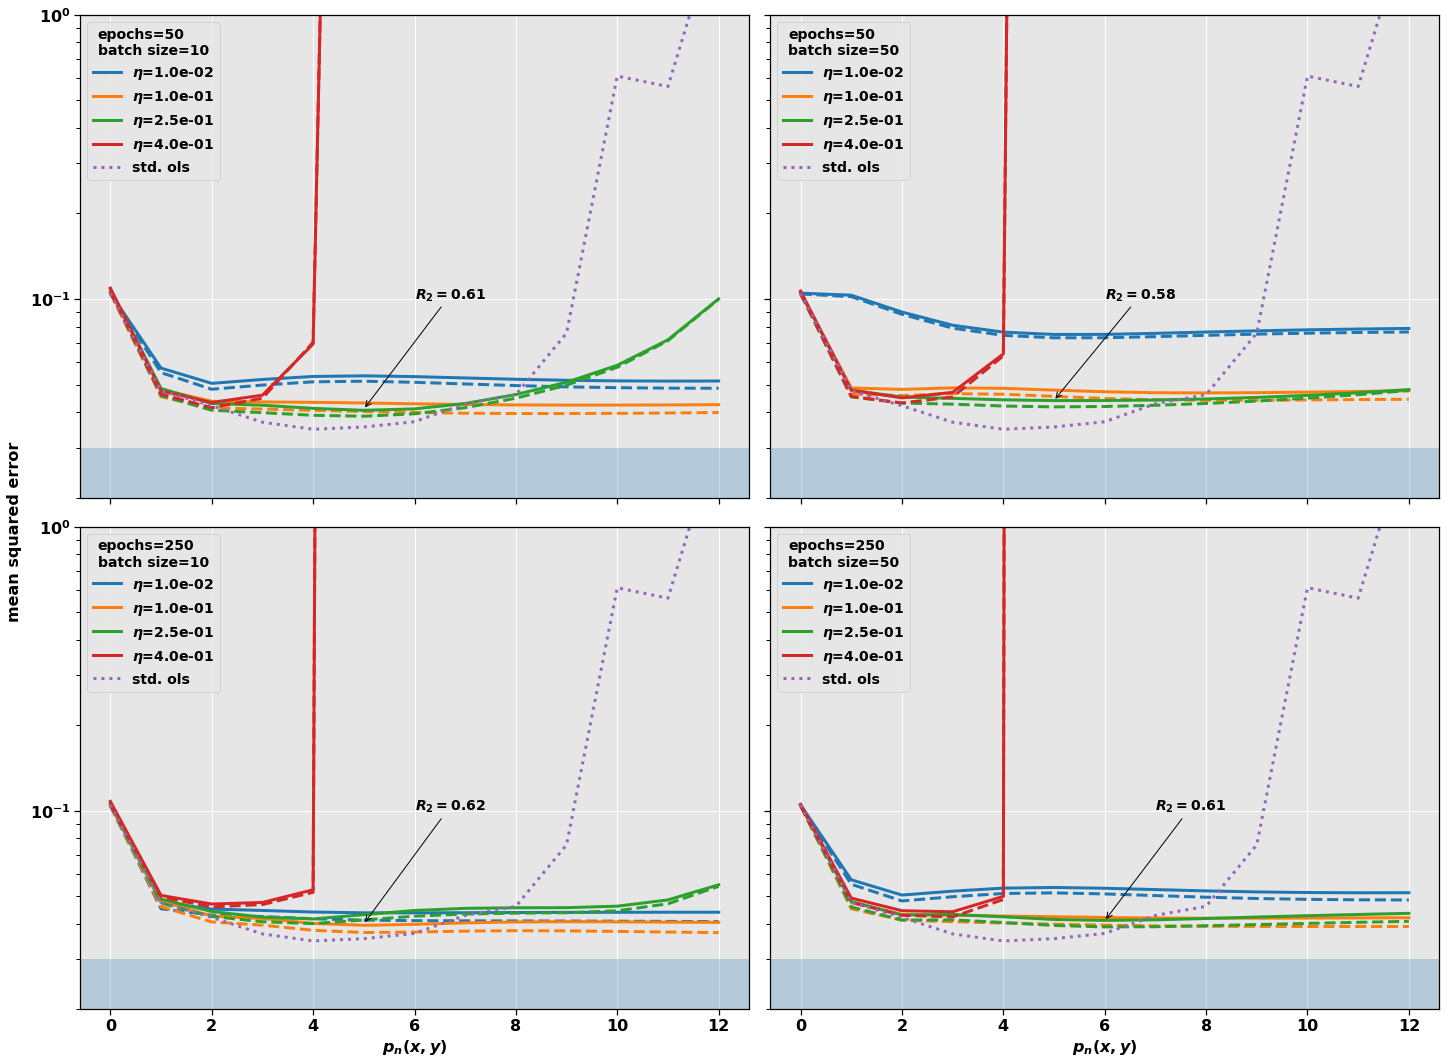
\includegraphics[width=1\linewidth]{ols_sgd.png}
	\caption{OLS with SGD on 250 randomly drawn samples generated by the Franke function. Test MSE in full-drawn lines for various learning rates $\eta$, and train MSE in dotted lines with colors for corresponding $\eta$. The blue-shaded area in each pane indicates the noise level in the samples. To the upper right we see that $\eta = 2.5 \cdot 10^{-1}$ bends steeply upwards after the best fit around $p_5(x,y)$. This tendency is damped by increasing either batch size or epochs. Overall, traditional OLS has better fit than OLS with SGD, as we see from the dotted purple line, which has $R_2 = 0.69$, but SGD prevents overfitting much in the same way as Ridge and LASSO.}
	\label{fig:ols_sgd}
\end{figure}

\begin{figure}[!htb]
	\centering
	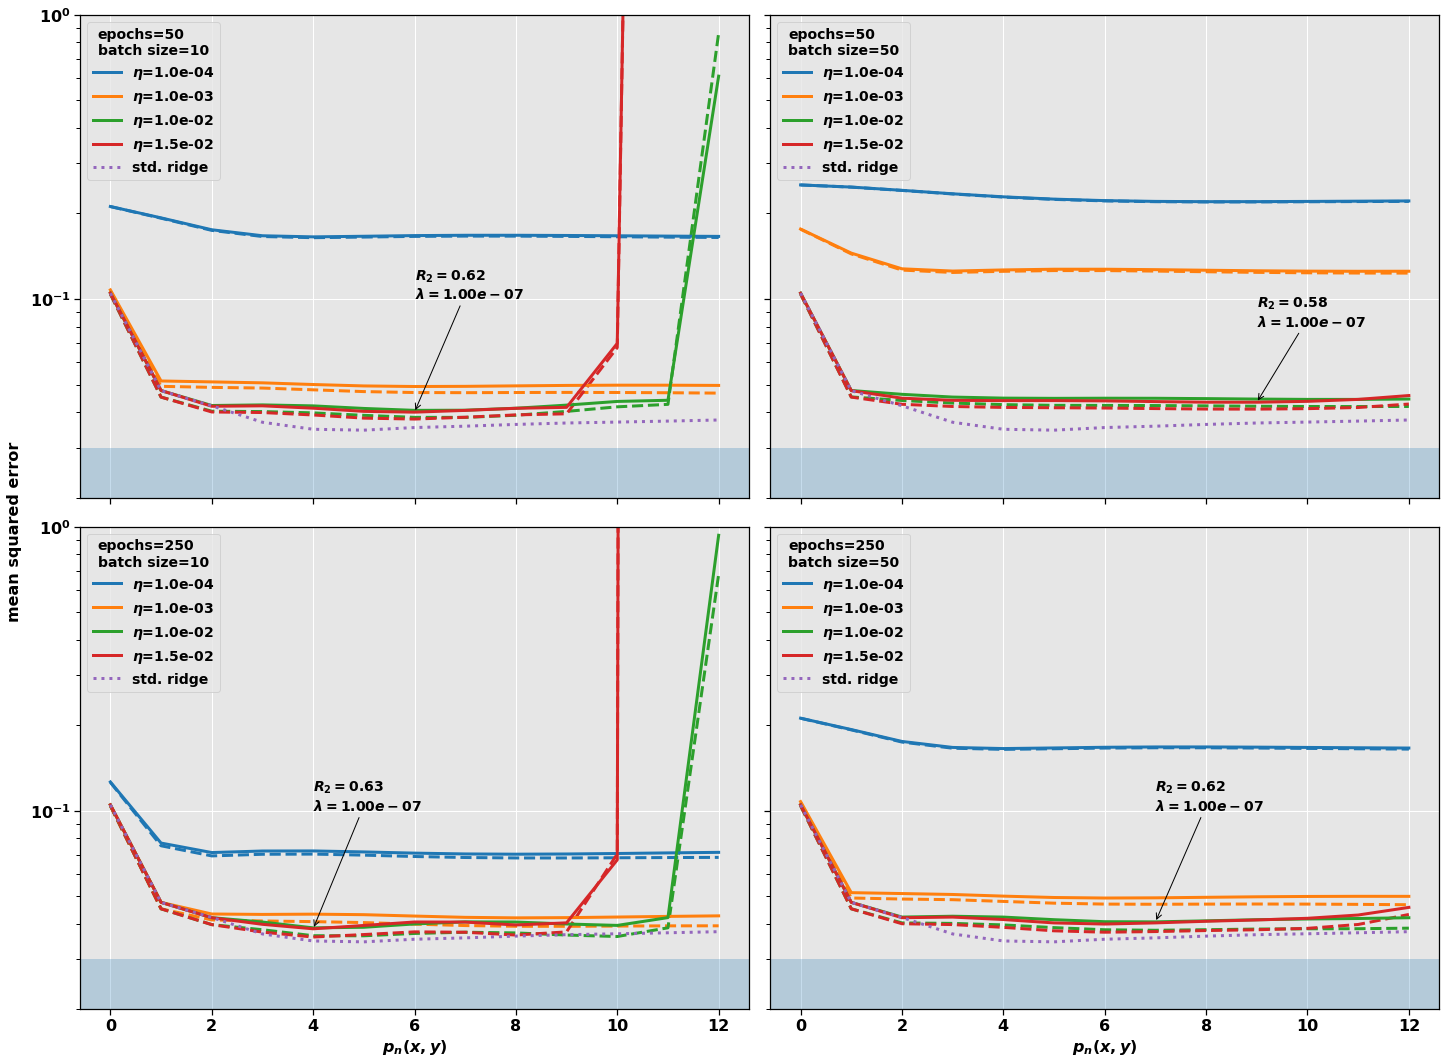
\includegraphics[width=1\linewidth]{ridge_sgd.png}
	\caption{Ridge with SGD on 250 randomly drawn samples generated by the Franke function. Test MSE in full-drawn lines for various learning rates $\eta$, and train MSE in dotted lines with colors for corresponding $\eta$. The blue-shaded area in each pane indicates the noise level in the samples. Ridge with SGD has approximately the same MSE/$R_2$ performance as OLS with SGD, but is more stable. The point at which the $\eta = 4.0 \cdot 10^{-1}$ model blows up in the 50 epochs cases is moved from the 5th to the 12th polynomial. The traditional Ridge regression method }
	\label{fig:ridge_sgd}
\end{figure}


\begin{figure}[!htb]
	\centering
	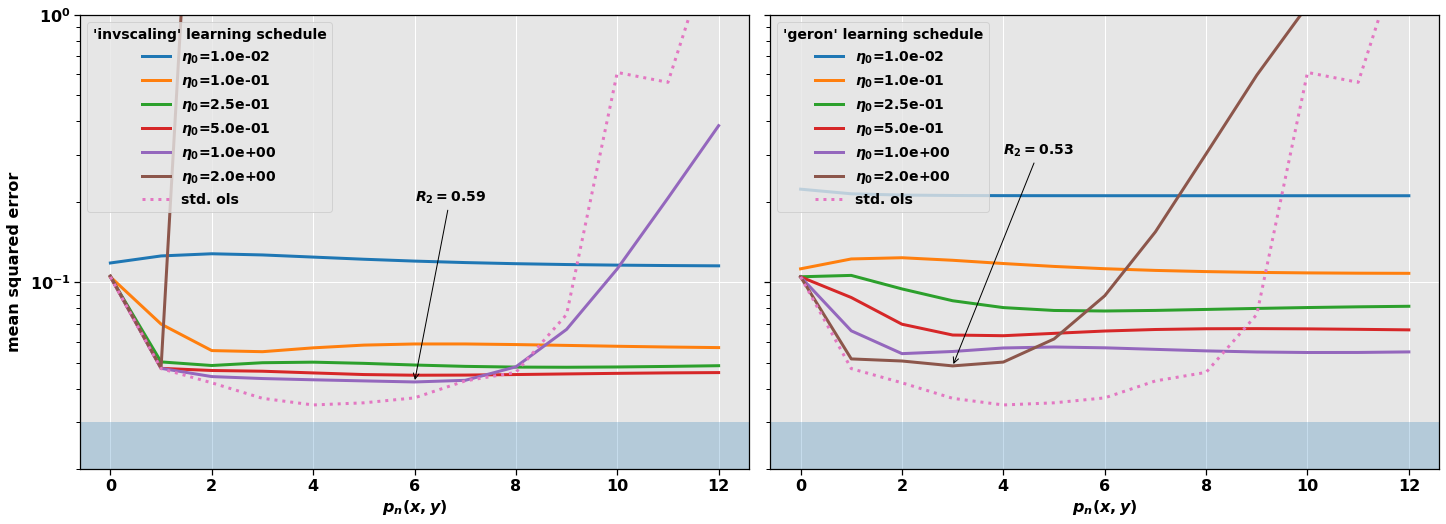
\includegraphics[width=1\linewidth]{ols_sgd_schedules.png}
	\caption{Two different learning schedules for OLS with SGD on the same data as in Figure \ref{fig:ols_sgd}, with 50 epochs and mini batch size 10. 'invscaling' (Equation (\ref{invscaling})) is initialized with $k=0.5$ and $\eta_0$, and 'geron' (Equation (\ref{geron})) is initialized with $t_0 = \eta_0$ and $t_1 = 1$. We see that a learning schedule lets us select larger values of $\eta_0$, and that it prevents the model from blowing up due to complexity. On this data set and with these parameters, 'invscaling' performs roughly as well as the 'constant' schedule, while 'geron' has poorer performance.}
	\label{fig:ols_sgd_schedules}
\end{figure}

\subsection{Regression with Feed-Forward Neural Network}
%Train your network and compare the results with those from your OLS and Ridge Regression codes from project 1. You should test your results against a similar code using Scikit-Learn

%Comment your results and give a critical discussion of the results obtained with the Linear Regression code and your own Neural Network code. Compare the results with those from project 1. Make an analysis of the regularization parameters and the learning rates employed to find the optimal MSE and R2 scores.

%You should now also test different activation functions for the hidden layers. Try out the Sigmoid, the RELU and the Leaky RELU functions and discuss your results. You may also study the way you initialize your weights and biases. 

The activation function in the output layer is the sigmoid function, which is limited to $[0,1]$. See Table \ref{tab:activation-funcs}. To approximate the response variables, we need to scale them to the same range $[0,1]$. We do this by first adding the minimum sample value to all response variables and then dividing by the maximum value. Likewise we have to center and scale the design matrix, since we will use $L_2$ regularization.

Figure \ref{fig:ffnn_reg_sigmoid} shows the $R_2$ scores for an $\eta$-vs-$\lambda$ grid search with a Feed-Forward Neural Network. We have used the same Franke function samples as in the preceding discussion on OLS and Ridge; 250 random samples with some noise. The design matrix is generated by a 12th degree polynomial in two variables, meaning that it has $p = 78$ features. The network thus has 78 nodes in the input layer, and we have used the same number in the single hidden layer. The hidden layer activation function is sigmoid, which is the same as the single-node output. We thus have 78+1 biases and 78*79 weights to determine, 6241 parameters all-in-all. The initialization is done by random values in the range $[0,1]$ for the weights, and the biases are all set to 0.01.

We see in the lower left pane of the figure that the best $R_2$ score 0.55 occurs for 250 epochs and mini batch size 10, with $\eta = 3.0$ and $\lambda = 1.0 \cdot 10^{-3}$. This is quite poor compared with the performance of OLS and Ridge in the previous section, and even poorer when compared with traditional OLS, which achieved an $R_2$ of 0.69. For the other sets of epochs and batch sizes, performance is quite low; barely tipping over $R_2 = 0$, which means that generally we would be better off by simply approximating the function by taking the mean of the samples.

The $R_2$ scores in Figure \ref{fig:ffnn_reg_sigmoid} vary widely for relatively short changes in the hyperparameters $\eta$ and $\lambda$. This suggests that the shape of the variable space which we are moving in is quite rugged, with many local minima and saddle points. There may well be better fits to be found, and changing the activation function may help with this. 

In Figure \ref*{fig:ffnn_reg_relus} two different activation functions have been tested on the same data and with 250 epochs, batch size 10, as gave the best fit for sigmoid. To the left we see the result of the ReLU activation function, and to the right the related leaky-ReLU. Again, see Table \ref{tab:activation-funcs}. ReLU has best performance for $\eta = 0.1-0.2$ and $\lambda=1.0 \cdot 10^{-2}$, where it gets an $R_2$ score of 0.56 -- marginally better than sigmoid's 0.55. Leaky-ReLU, on the other hand, achieves a comparable $R_2$ of 0.55 at $\eta = 3.0$ and $\lambda=1.0 \cdot 10^{-3}$, so the small difference between the two functions gives a relatively large impact in the hyperparameters.

\begin{figure}[!htb]
	\centering
	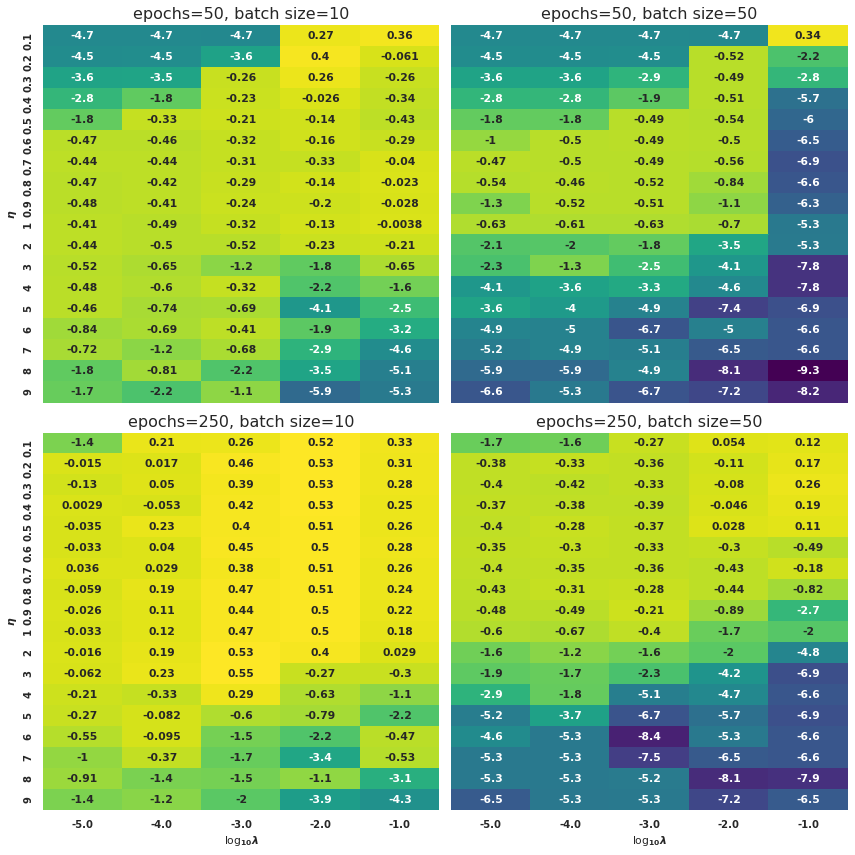
\includegraphics[width=1\linewidth]{ffnn_reg_sigmoid.png}
	\caption{$R_2$ scores on the Franke function after $\eta$-vs-$\lambda$ grid search with a Feed-Forward Neural Network. The network has a single hidden layer with sigmoid activation function. The network has been trained on 250 samples and 5-fold cross validation, with varying number of epochs and mini batch size in each pane. The best score $R_2=0.55$ is somewhat poorer than the score obtained with OLS and Ridge.}
	\label{fig:ffnn_reg_sigmoid}
\end{figure}

\begin{figure}[!htb]
	\centering
	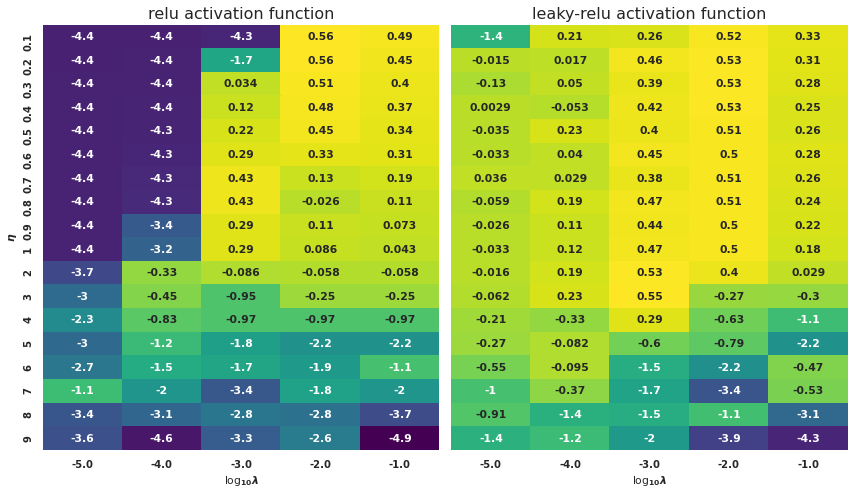
\includegraphics[width=1\linewidth]{ffnn_reg_relus.png}
	\caption{$R_2$ scores on the Franke function after $\eta$-vs-$\lambda$ grid search the same Feed-Forward Neural Network as in Figure \ref{fig:ffnn_reg_sigmoid}, but with ReLU and leaky-ReLU activation functions in the hidden layer instead of sigmoid. Epochs is 250 and mini batch size 10. The performance of the ReLU functions is comparable with that of sigmoid, but has a large influence on the choice of hyperparameters.}
	\label{fig:ffnn_reg_relus}
\end{figure}

\subsection{Classification with Feed-Forward Neural Network}
%We will here study the MNIST data set of hand-written numbers. Use the Softmax function as activation function. Your code should however also be able to use a binary activation function as well. 

%Discuss your results and give a critical analysis of the various parameters, including hyper-parameters like the learning rates and the regularization parameter λ (as you did in Ridge Regression), various activation functions, number of hidden layers and nodes and activation functions. 

We will now study how our Feed-Forward Neural Network performs on classification problems. Let's start with binomial classification using the Wisconsin Breast Cancer dataset, available through Python's \lstinline|sklearn| module \cite{skl-datasets}. The dataset contains 569 samples with 30 features characterizing breast cancers. See Figure \ref{fig:log_breast_cancer_bars} further down. The design matrix will consist of 30 features, and the response variables will be contained in a vector of length 569, with 1s and 0s. 

Of the 569 samples, 357 are \text{positive} indications for breast cancers, meaning that a strategy of guessing only 1s would yield an \textit{accuracy} of about 63 \%. 63 \% must thus serve as a baseline when we evaluate the accuracy of our model.

It proved difficult to train an FFNN with one hidden layer to fit to the breast cancer dataset. Therefore, what we will use is 30 nodes in the input layer directly connected to the output layer, building what is known as a \textit{perceptron} model. The perceptron has a unit-step activation function (see Table \ref{tab:activation-funcs}).

In Figure \ref{fig:ffnn_breast_cancer} we see the result of a $\eta$-vs-$\lambda$ grid search on the perceptron model. We see that for 250 epochs and batch size 10 it has 95 \% accuracy, meaning that it performs quite well compared to the 63 \% baseline. There is not very much variation for other numbers of epochs and batch sizes, and the model is not very sensitive to the learning rate and $L_2$ regularization parameter. This indicates that the perceptron model is stable and reliable when applied to this data set.

\vspace{5mm}

Next, let's evaluate our FFNN's performance on \lstinline|sklearn|'s reduced version of the MNIST dataset of handwritten numbers 0 to 9 \cite{skl-datasets}. The full, more expansive dataset is freely available from from the MNIST website at. See \cite{mnist}. Some samples from the dataset which we will use here are shown in Figure \ref{fig:mnist_digits}. 

The dataset contains 1797 pictures, each with $8 \times 8$ pixels with a numerical value 0 to 16. The design matrix thus has shape $1797 \times 64$, and the one-hot representation of the reponse variables becomes a $1797 \times 10$ matrix with a single 1 in each row, and the rest 0s.

The network must therefore have 64 input nodes, and we have selected equally many nodes in the hidden layer, which we activate by the sigmoid. The output layer has one node for each of the 10 classes of outcomes and has softmax activation function, which ensures convergence towards one output for each 64-feature input sample. The system has 4810 weights and biases to train.

Figure \ref{fig:ffnn_digits} shows the result of the $\eta$-vs-$\lambda$ grid search. We see that for $\eta = 1.0 \cdot 10^{-2}$ and $\lambda = 1.0 \cdot 10^{-1}$, accuracy lies at 0.97 to 0.98 for all the selected numbers of epochs and batch sizes and that the accuracy is quite good in an area around these $\eta$ and $\lambda$ values, especially for the 250 epochs and 10 batch size case. As for the perceptron in the binomial case, this indicates that the model is stable and suitable for making predictions on this dataset.

The comparable performance for \lstinline|sklearn.neural_network.MPLClassifier| is about 99 \%.

\begin{figure}[!htb]
	\centering
	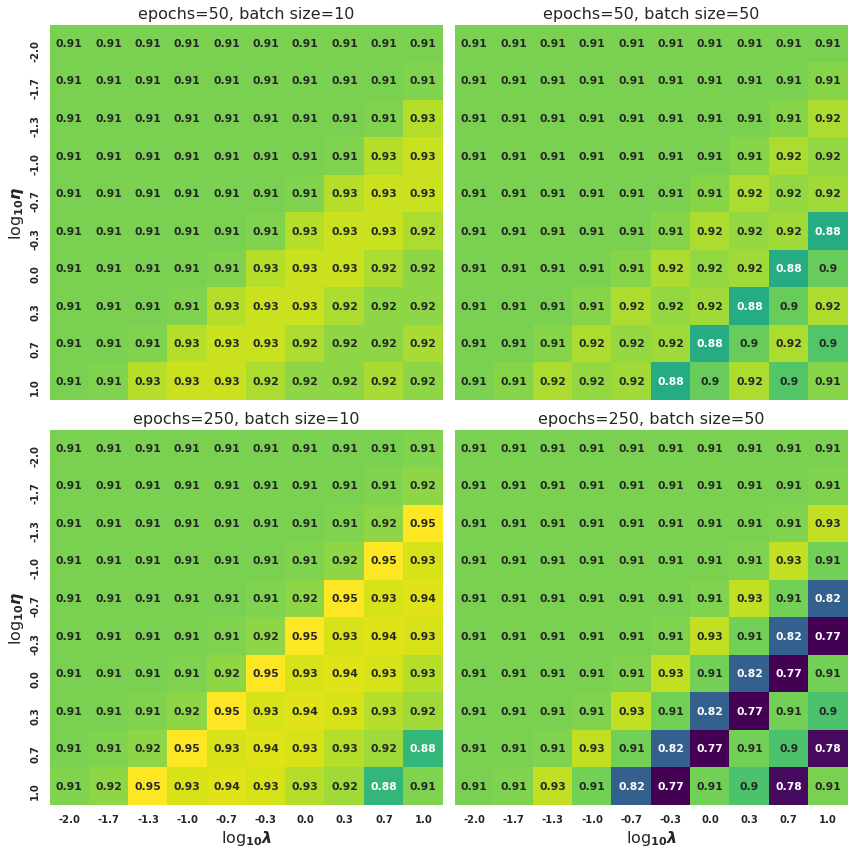
\includegraphics[width=1\linewidth]{ffnn_breast_cancer.png}
	\caption{Feed-Forward Neural Network as perceptron model (no hidden layer). The panes show the result of $\eta$-vs-$\lambda$ grid searches for different numbers of epochs and mini batch sizes. The baseline accuracy (predict only 1s) is 63 \%, and we achieve 95 \% with this perceptron model. Activation function is the unit-step, and learning schedule 'geron' with $t_0 = \eta$ and $t_1 = 1$ (see Equation (\ref{geron})).}
	\label{fig:ffnn_breast_cancer}
\end{figure}


\begin{figure}[!htb]
	\centering
	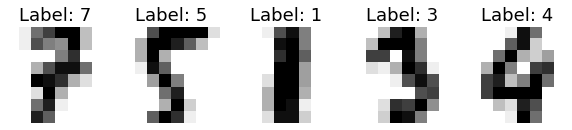
\includegraphics[width=1\linewidth]{mnist_digits.png}
	\caption{Some samples from the reduced MNIST dataset available through the \lstinline|sklearn| Python module. Each picture contains one handwritten figure and has $8 \times 8$ pixels.}
	\label{fig:mnist_digits}
\end{figure}

\begin{figure}[!htb]
	\centering
	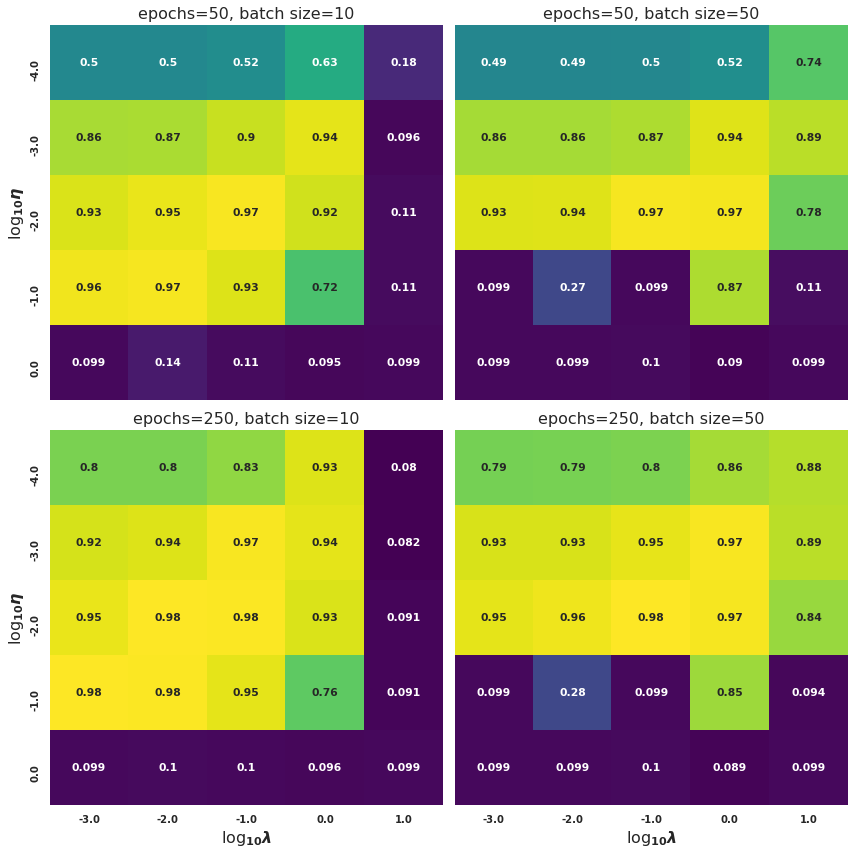
\includegraphics[width=1\linewidth]{ffnn_digits.png}
	\caption{Prediction accuracy results of a FFNN on the \lstinline|sklearn| MNIST dataset. The network has one hidden layer activated by the softmax function. Learning schedule is 'constant'. We see that the accuracy is quite stable around 0.97 to 0.98 for the best $\eta$ and $\lambda$ values.}
	\label{fig:ffnn_digits}
\end{figure}

\subsection{Logistic Regression}
%Study the results as functions of the chosen learning rates. Add also an l2 regularization parameter λ. Compare your results with those from your FFNN code as well as those obtained using Scikit-Learn's logistic regression functionality. 

In contrast to ANNs, logistic regression produces a prediction model which gives insight into the data which we have fed into it. The coefficient variables $\beta_j$ tells us each associated feature's influence on the prediction per unit change at the input. 

Keeping that in mind, Figure \ref{fig:log_breast_cancer_bars} shows the positive and negative predictive value of each of the features in the Wisconsin Breast Cancer data set \cite{skl-datasets}. Note that the features have not been scaled prior to the generation of this chart, so the unit of input must be considered, but on a logarithmic scale the higher bars are likely to have the strongest predictive value, such as 'area error' and 'worst area' for the positive predictors, and 'mean perimeter' and 'worst perimeter' for the negative. The meaning of each of these should better be considered by a professional, but the 'intercept' gathers the variation in the output which is not explained by the other features -- 'bad luck' in this case, it would seem.

Figure \ref{fig:log_breast_cancer} shows logistic regression's train and test accuracy in a $\eta$-vs-$\lambda$ grid search. Here, the design matrix has been centered and scaled. We see that the test accuracy follows the train accuracy very closely, and reaches 98 \% at $\eta = 1.0 \cdot 10^{-2}$. What is also noticeable is that it is seemingly insensitive to $L_2$ regularization, both in the training and testing cases. Number of epochs is 100 and mini batch size 10 in the results presented here, but changing this did not change the result significantly. 

Compared to the accuracy of the perceptron model (FFNN without hidden layer) presented above, logistic regression performs better. With the neural network we achieved 95 \% accuracy at the best, 3 percentage point lower than here. 

\vspace{5mm}

At last, let's investigate the performance of logistic regression on \lstinline|sklearn|'s MNIST dataset \cite{skl-datasets}, as we did for FFNN. We will not present a bar chart of the coefficient estimates, since that information probably is not very telling, but the results of the $\eta$-vs-$\lambda$ grid search is shown in Figure \ref{fig:log_digits}. As for the breast cancer dataset, the train accuracy is closely followed by the test accuracy, and again we see that the model is insensitive to variations in $\lambda$, which again is surprising. The test accuracy reaches 94 \% at $\eta = 1.0 \cdot 10^{-1}$. This is poorer than the performance of the neural network, which reached all the way to 98 \%. However, the result shows that logistic regression clearly would find its use for this type of problem. Again, as for the breast cancer dataset, number of epochs is 100 and mini batch size 10 in the results presented here. Changing these values did not change the result significantly. 

\begin{figure}[!htb]
	\centering
	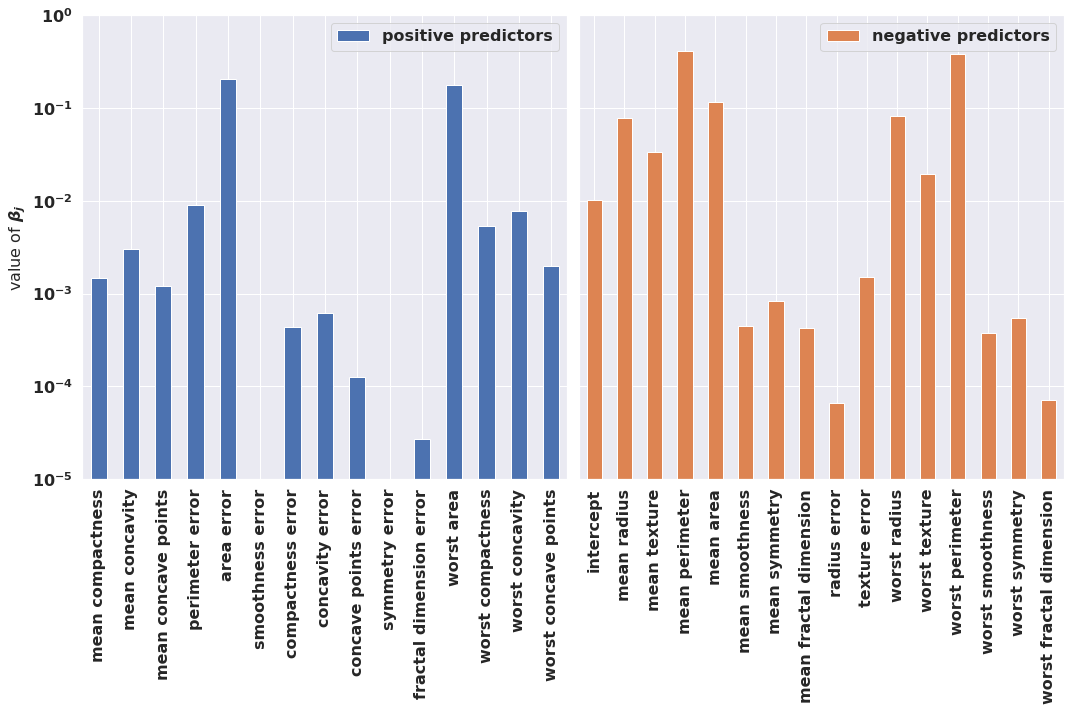
\includegraphics[width=1\linewidth]{log_breast_cancer_bars.png}
	\caption{Logistic regression on the binomial Wisconsin Breast Cancer dataset available from \lstinline|sklearn|. The bars show the coefficient estimates $\beta_j$ for positive predictors to the left and negative to the right. Regression was made on unscaled data, with 100 epochs, batch size 10 and $\eta = 1.0 \cdot 10^{-4}$, which gives a prediction accuracy of 97 \%. The higher the bar, the higher the predictive value, but on a per-unit input base, since the data was unscaled when the model was generated.}
	\label{fig:log_breast_cancer_bars}
\end{figure}


\begin{figure}[!htb]
	\centering
	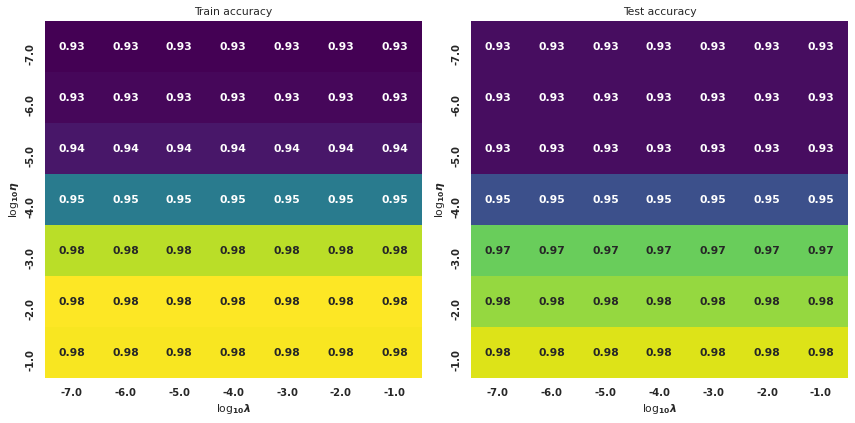
\includegraphics[width=1\linewidth]{log_breast_cancer.png}
	\caption{Logistic regression on the binomial Wisconsin Breast Cancer dataset available from \lstinline|sklearn|. Training was done with 100 epochs and batch size 10, and with 'constant' learning schedule. Train accuracy to the left is followed closely by the test accuracy to the right. The model is seemingly insensitive to the $L_2$ regularization parameter $\lambda$. Logistic regression performs better than the perceptron model on this dataset.}
	\label{fig:log_breast_cancer}
\end{figure}

\begin{figure}[!htb]
	\centering
	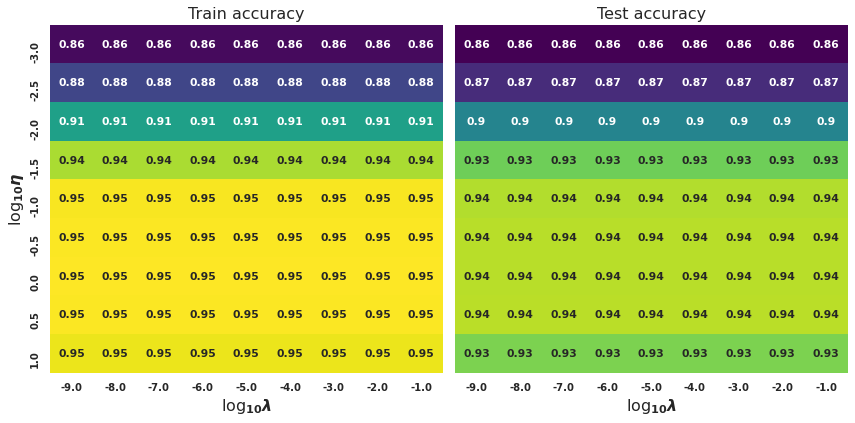
\includegraphics[width=1\linewidth]{log_digits.png}
	\caption{Logistic regression on the multinomial MNIST dataset available from \lstinline|sklearn|. Training was done with 100 epochs and batch size 10, and with 'constant' learning schedule. Train accuracy to the left is followed closely by the test accuracy to the right. The model is seemingly insensitive to the $L_2$ regularization parameter $\lambda$. FFNN with one hidden layer performs better than logistic regression on this dataset.}
	\label{fig:log_digits}
\end{figure}


\clearpage
\section{Discussion and Conclusion} \label{conclusion}
% - State your main findings and interpretations
% - Try as far as possible to present perspectives for future work
% - Try to discuss the pros and cons of the methods and possible improvements

We have seen that linear regression solved with SGD performs worse than the traditional OLS and Ridge methods with matrix inversion. However, SGD has some of the same qualities as Ridge and LASSO in that it prevents overfitting of the model, which allows us to increase model complexity beyond the point where OLS blows up. Linear regression with OLS may also blow up when we pick a learning rate and gradually increase model complexity, but not necessarily due to overfitting. The model becomes unstable because the maximum eigenvalue of the Hessian matrix, $\lambda_{max}$, increases in value as the model complexity increases, which lets the model blow up when $\eta \ge 2/\lambda_{max}$. For linear regression, the Hessian matrix is given by $\mathbf{H} = \mathbf{X}^\intercal \mathbf{X} + \lambda \mathbf{I}$, and this addition of the $L_2$ regularization parameter $\lambda$ reduces $\lambda_{max}$, which allows us to increase the learning rate. A very clear indication of this is the tendency of the train and test MSEs to follow each other closely, also after the model blows up. This shows that the model does not suffer from overfitting.

As for the linear regression with SGD, our neural network also performed quite poorly on the regression problems that we have studied -- worse than linear regression with SGD. This might be for many reasons; non-optimal selection of hyperparameters such as number of epochs, batch size, regularization, learning rate or learning schedule. We studied some of these, but in addition we could also tweak the initialization of biases and weights (which we didn't touch at all), further investigate a mix of activation functions, and of course the network's architecture. The potential for optimization seems to be almost infinite, and therefore beyond what we would investigate in this report.

We have shown that the Feed-Forward Neural Network developed for this report could be used successfully for perceptron modelling with unit-step activation. The derivative of the unit-step, which in reality is always zero (except for at zero), could be approximated by the unit-step itself. The performance on the Wisconsin Breast Cancer dataset \cite{skl-datasets} was somewhat below that of logistic regression, though.

Where the FFNN did excel was when it was applied on the multinomial classification problem with the simplified MNIST dataset \cite{skl-datasets}. It reached 98 \% accuracy, which was ascertained by 5-fold cross validation.

On the multinomial problem, logistic regression also performed well, however. And, importantly, training a relatively shallow and narrow neural network on even a quite limited dataset such as this (1797 samples with 64 features) takes is computationally demanding. Here, logistic regression with SGD has a great advantage, provided that the decision boundary is linear, of course.

Another advantage of logistic regression over neural networks is that it generates a model which is interpretable for the human, as we saw for the breast cancer data. Logistic regression gave very valuable insights about the data that we fed into it.

\vspace{5mm}

The most important suggestion for future studies is to investigate the insensitivity to $L_2$ regularization, which we observed for logistic regression. This may very well stem from an error in my implementation of the algorithm; or some other phenomena which I did not manage to identify.

Further, the neural network's poor performance on the regression problem came as a bit of a surprise. Further insights into the reason for this would be valuable.

\clearpage
\bibliographystyle{unsrt}
\bibliography{project2.bib}
\end{document}
